\section{使用\keyword{nano}简单创建文件}\label{sec:使用nano简单创建文件}
\sectionAuthor{Jiaqi Z.}

\begin{Abstract}
    \item 如何使用\code{nano}创建并编辑文本文件
\end{Abstract}

在第\ref{chap:Linux命令行操作}章当中,已经了解了如何对Linux进行基本的操作,例如查看目录、移动或删除文件等,同时在\ref{sec:文件权限管理}一节讨论了如何给文件添加权限,例如,给脚本程序添加可执行权限。

然而,我们在Linux的所有对文件的操作,目前只限于\emph{读取},对于编辑,目前所采用的方法是将其保存至Windows下,利用记事本等软件进行编辑,完成后再上传回Linux系统。然而,无论是使用Linux本地操作系统,还是在服务器上使用,如果可以在系统中直接编辑文件,显然更方便\footnote{虽然在VS Code当中,也许可以如同本地文件一般编辑服务器上的文件,但作为Linux教程,我们还是会尽可能介绍普遍适用的方法。}。在本章,我们将详细介绍Linux下如何编辑文件。

目前,Linux最常用的文本编辑器是vi和vim,而在这之前,我们先介绍一个更简单的文本编辑器--\code{nano}。相比于vi和vim,\code{nano}功能可能会更少,但是作为开始Linux文件编辑的第一步,也许是合适的。

\begin{extend}
    在很多时候,我们会把vi和vim放在一起讨论。它们具有类似的界面,类似的工作模式,因此很多人容易将其混为一谈。实际上,vi是由Bill Joy在1976开发的一款Unix操作系统下的可视化编辑器(Linux是1991年诞生的);而vim是Bram Moolenaar在1991年开发的vi改进版(Vi improved),其功能包含语法高亮、插件支持等。

    虽然我们经常在Linux当中使用vim,但它本身是可以跨平台运行的,如Windows本身也是可以安装支持vim。只不过由于Windows本身的文本编辑软件足够丰富,同时大多数Windows用户并不熟悉命令行操作本身。因此,很多人也是在接触Linux的时候第一次接触vim编辑器。

    关于二者之间的更多区别,可以查看网址:\\https://blog.csdn.net/weixin\_53269650/article/details/138137434
\end{extend}

\subsection{使用\code{nano}创建第一个文件}\label{subsec:使用nano简单创建文件-使用nano创建第一个文件}

使用\code{nano}命令非常简单,通常只需要使用\code{nano <要打开的文件路径名>},对于不存在的文件,它会自动创建一个;而已经存在的文件则会将其打开。

例如,在家目录下,我们直接创建一个名为\code{hello}的文件。使用命令\code{nano hello},则会进入nano编辑器的模式。如果你用过老式操作系统,则会发现这个界面十分“复古”--上面是编辑区,下面是一些选项(类似于Windows软件的“菜单”)如图\ref{fig:使用nano简单创建文件-nano界面}所示。

\begin{figure}
    \centering
    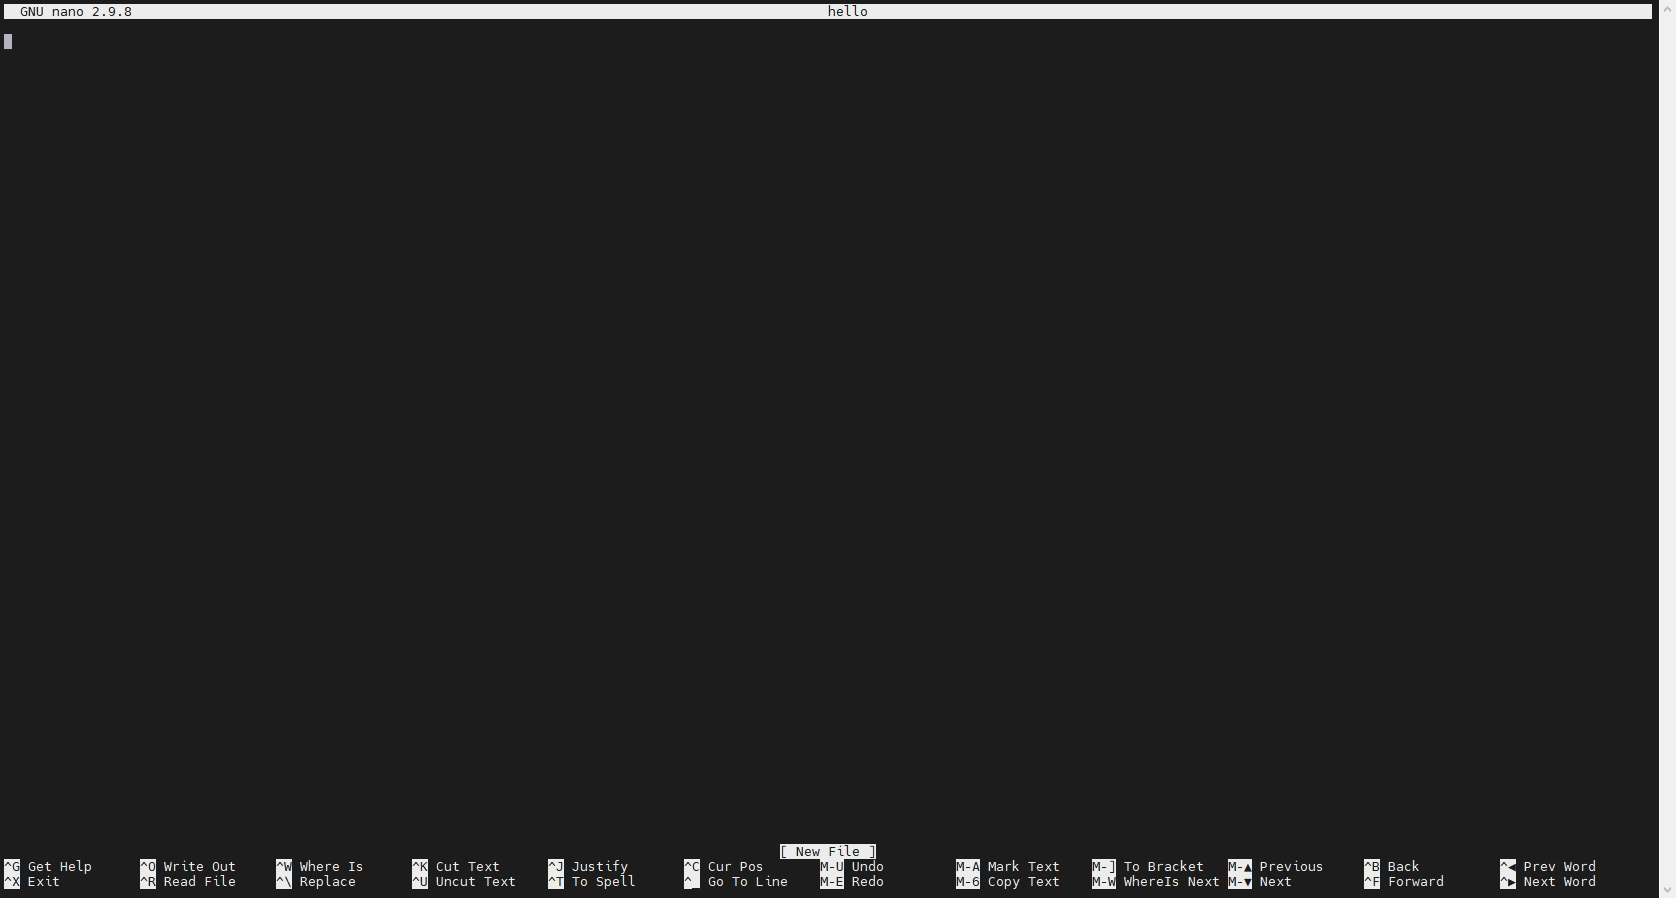
\includegraphics[width=1\linewidth]{Linux基础/文本编辑工具vi和vim/使用nano简单创建文件/fig/nano界面.png}
    \caption{nano界面}
    \label{fig:使用nano简单创建文件-nano界面}
\end{figure}

当打开时,软件默认就是\emph{编辑模式},你可以在里面随意输入一些内容,例如,输入“hello world”,屏幕上就是直接显示你的内容。对于删除和换行,其操作就如图在Windows下的记事本一样(使用键盘上下左右、删除键等)。重点是下面的菜单选项。难度本身也不大,只需要记住两个符号所表示的含义即可:\^表示键盘上的\code{Ctrl}键,而\code{M-}表示键盘上的\code{Alt}键。因此,正如你所看到的那样,在nano当中,使用\keywordin{nano}{Ctrl+X}退出;使用\keywordin{nano}{Ctrl+O}保存。

\begin{attention}
    在\code{nano}当中,一个很特殊的地方在于它的复制、剪切和粘贴与我们所熟悉的快捷键不一样。根据下面的说明,可以看到,复制是\keywordin{nano}{Alt+6},剪切是\keywordin{nano}{Ctrl+K},而粘贴是\keywordin{nano}{Ctrl+U}。

    同时,无论是复制还是剪切,默认都是\emph{对行进行操作}。也可以使用\keywordin{nano}{Alt+A}\footnote{这个命令可能和部分软件(如微信)的截图快捷键冲突。},并用方向键选中文本,进行操作。
\end{attention}

此外,\code{nano}也支持撤销(\keywordin{nano}{Alt+U})和恢复(\keywordin{nano}{Alt+E})。

\subsection{使用\code{nano}进行查找和替换}

几乎所有的文本编辑器,都需要有一些如\emph{查找}和\emph{替换}的功能方便我们进行编辑。在\code{nano}当中,查找的命令是\keywordin{nano}{Ctrl+W},此时下方会弹出一个输入框,输入要查找的内容,回车后光标便会定位在光标下方第一个匹配的开头位置。使用\keywordin{nano}{Alt+↓}和\keywordin{nano}{Alt+↑}可以切换到下一个匹配位置或上一个匹配位置。

\begin{attention}
    \code{nano}在匹配查找时不区分大小写,例如,想查找\code{SIGMA}时,在输入查找内容时输入\code{sigma}同样可以。
\end{attention}

对于替换功能,其命令为\keywordin{nano}{Ctrl+$\backslash$},此时首先弹出对话框,输入要查找的内容的,之后弹出的对话框输入要替换的内容。之后光标会从当前位置开始向后搜索,当查找到一个后会定位到此处并询问是否替换。输入\code{y}表示确认,输入\code{n}表示不替换此处。如果确认要全部替换的话,可以直接输入\code{a};相对地,如果发现有错(例如要查找的词语或要替换的词语拼写错了),可以输入\code{c}取消替换命令。

除此之外,还有更多的命令(例如查看字数是\keywordin{nano}{Alt+D}),可以直接使用\keywordin{nano}{Ctrl+G}查看帮助文档。在帮助文档中还包含有一些命令的快捷方式,例如查看文档除了可以使用\code{Ctrl+G}外,也可以直接使用\code{F1}键。

\begin{attention}
    \code{nano}的使用方法看似讲了很多,实际上只需要记住:\^表示键盘上的\code{Ctrl}键,而\code{M-}表示键盘上的\code{Alt}键,其他的,都可以通过下方的说明,或者帮助文档找到。
\end{attention}

\subsection{错误处理}\label{subsec:使用nano简单创建文件-错误处理}

\subsubsection{[ File <文件名> is unwritable ]}

这是因为你没有这个文件的可编辑权限。借助于\ref{subsec:文件权限管理-修改文件权限}一节所介绍的\code{chmod}命令可以添加可编辑权限。

\begin{attention}
    大多数时候,之所以这个文件不可编辑,是因为这个文件含有重要内容(可能是你误打了一个系统文件的路径,虽说这个可能性很小)。因此,遵守这个权限,不要修改是最好的。如果确实需要修改,仔细检查。
\end{attention}

\subsubsection{[ Error reading <文件名>: Permission denied ]}

这是因为你没有这个文件的可读权限,解决方法与上一个错误一样(使用\code{chmod}命令)

与前面的注意内容一样,遵守这个权限往往是最正确的选择。